\documentclass[tikz,margin=3mm]{standalone}
\usepackage[utf8]{inputenc}
\usepackage[T1]{fontenc}
\usepackage{tikz}
\usetikzlibrary{shapes.geometric, arrows.meta, positioning, calc, fit, backgrounds}
\usepackage{xcolor}
\definecolor{primary}{HTML}{1B75BC}
\definecolor{secondary}{HTML}{F15A29}
\definecolor{accent}{HTML}{8CC63F}
\definecolor{grayC}{HTML}{4D4D4D}
\definecolor{graylight}{HTML}{F2F2F2}
\definecolor{blueC}{HTML}{1B75BC}
\definecolor{orangeC}{HTML}{F15A29}
\definecolor{yellowC}{HTML}{FBB03B}
\definecolor{purpleC}{HTML}{92278F}

\tikzset{
  base/.style={rectangle, rounded corners=4pt, draw=grayC, minimum width=3.5cm, minimum height=1cm, align=center, font=\footnotesize, fill=white, line width=0.8pt},
  ndBlue/.style={base, draw=blueC, fill=blueC!8, text=primary},
  ndOrange/.style={base, draw=orangeC, fill=orangeC!8, text=primary},
  ndGreen/.style={base, draw=accent, fill=accent!8, text=primary},
  ndYellow/.style={base, draw=yellowC, fill=yellowC!8, text=primary},
  ndPurple/.style={base, draw=purpleC, fill=purpleC!8, text=primary},
  db/.style={cylinder, draw=grayC, shape border rotate=90, aspect=0.25, fill=graylight, minimum width=2.5cm, minimum height=1.5cm, align=center, font=\footnotesize, line width=0.8pt},
  arw/.style={->, >=stealth, line width=0.8pt, draw=grayC},
  lbl/.style={font=\scriptsize, fill=white, inner sep=2pt},
  bxBlue/.style={rectangle, rounded corners=6pt, draw=blueC, fill=blueC!3, dashed, inner sep=15pt},
  bxGreen/.style={rectangle, rounded corners=6pt, draw=accent, fill=accent!3, dashed, inner sep=15pt},
  bxPurple/.style={rectangle, rounded corners=6pt, draw=purpleC, fill=purpleC!3, dashed, inner sep=15pt},
  bxOrange/.style={rectangle, rounded corners=6pt, draw=orangeC, fill=orangeC!3, dashed, inner sep=15pt},
  lB/.style={font=\small\bfseries, text=blueC},
  lG/.style={font=\small\bfseries, text=accent},
  lP/.style={font=\small\bfseries, text=purpleC},
  lO/.style={font=\small\bfseries, text=orangeC}
}

\begin{document}
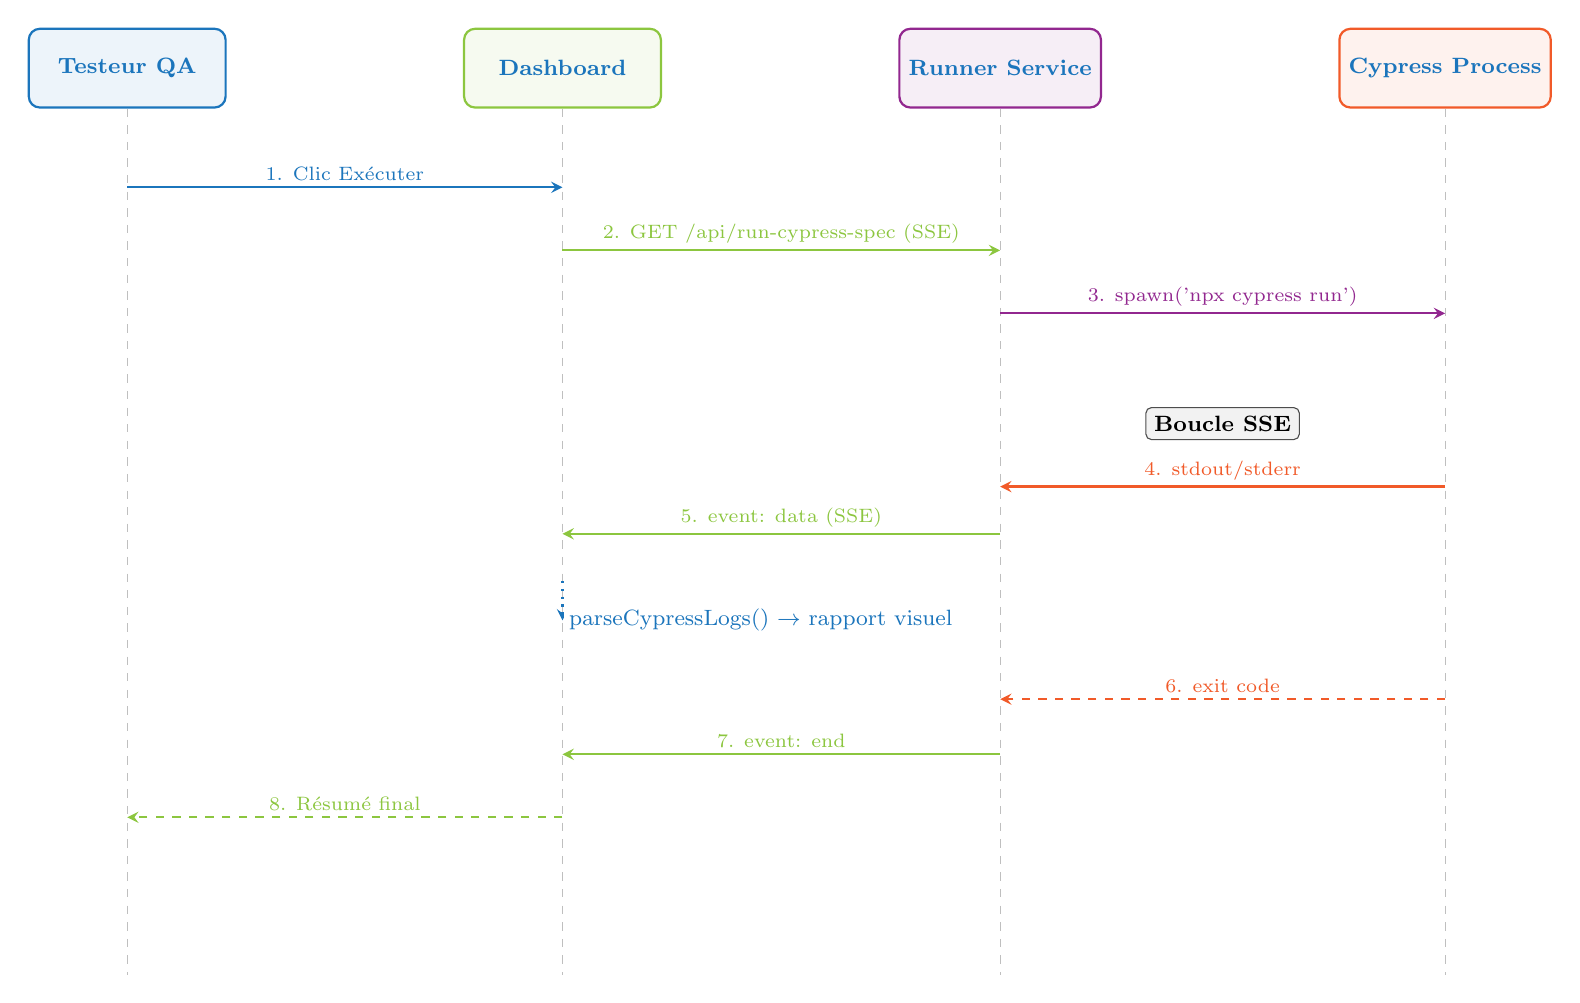
\begin{tikzpicture}
  % ── Lifelines ──
  \node[ndBlue, minimum width=2.5cm] (user2) {\textbf{Testeur QA}};
  \node[ndGreen, minimum width=2.5cm, right=3cm of user2] (dash2) {\textbf{Dashboard}};
  \node[ndPurple, minimum width=2.5cm, right=3cm of dash2] (runner2) {\textbf{Runner Service}};
  \node[ndOrange, minimum width=2.5cm, right=3cm of runner2] (cypress2) {\textbf{Cypress Process}};

  \foreach \n in {user2,dash2,runner2,cypress2}
    \draw[dashed, gray!50] (\n.south) -- ++(0,-11);

  \draw[arw, blueC] ([yshift=-1cm]user2.south) -- node[lbl, above]{1. Clic Exécuter} ([yshift=-1cm]dash2.south);
  \draw[arw, accent] ([yshift=-1.8cm]dash2.south) -- node[lbl, above]{2. GET /api/run-cypress-spec (SSE)} ([yshift=-1.8cm]runner2.south);
  \draw[arw, purpleC] ([yshift=-2.6cm]runner2.south) -- node[lbl, above]{3. spawn('npx cypress run')} ([yshift=-2.6cm]cypress2.south);

  % ── SSE Loop ──
  \node[rectangle, rounded corners=2pt, draw=grayC, fill=graylight, inner sep=3pt] at ([yshift=-4cm]$(runner2.south)!0.5!(cypress2.south)$) {\footnotesize\textbf{Boucle SSE}};
  \draw[arw, orangeC] ([yshift=-4.8cm]cypress2.south) -- node[lbl, above]{4. stdout/stderr} ([yshift=-4.8cm]runner2.south);
  \draw[arw, accent] ([yshift=-5.4cm]runner2.south) -- node[lbl, above]{5. event: data (SSE)} ([yshift=-5.4cm]dash2.south);
  \draw[arw, blueC, dotted] ([yshift=-6cm]dash2.south) -- ++(0,-0.5) node[lbl, right]{\footnotesize parseCypressLogs() $\rightarrow$ rapport visuel};

  % ── End ──
  \draw[arw, orangeC, dashed] ([yshift=-7.5cm]cypress2.south) -- node[lbl, above]{6. exit code} ([yshift=-7.5cm]runner2.south);
  \draw[arw, accent] ([yshift=-8.2cm]runner2.south) -- node[lbl, above]{7. event: end} ([yshift=-8.2cm]dash2.south);
  \draw[arw, accent, dashed] ([yshift=-9cm]dash2.south) -- node[lbl, above]{8. Résumé final} ([yshift=-9cm]user2.south);
\end{tikzpicture}
\end{document}
